\chapter{Results}
    \label{cha:results}
    %

    %
    \section{Bistability without cooperative enzymes}
        \label{sec:ResNon-cooperative}
        %

        %
        In this section, we consider systems which do not contain directly cooperative enzymes. Thus, all the enzymes in the system's rule set read at most one “read-only” nucleosome with a maximum space of zero from the nucleosome that is modified. The enzymes act on a non-cyclic nucleosome string.
        %

        %
        \subsection{Influence of noise}
            %
            As pointed out before, systems without cooperative enzymes can indeed be bistable. However, they are very sensitive to increased noise. This is illustrated in fig. \ref{img:nonCoopSim}. The enzymes featured in this system with their respective association rates are summarized in tab. \ref{img:enzymeRatesNoise}.
            %

            %
            \begin{table}[htbp!]
                \caption{Enzyme types that are included in the rule set for the run illustrated in fig. \ref{img:nonCoopSim} with their respective association rates. All enzymes' dissociation rates are at an equal rate of 100,000. The enzyme rule set is symmetrical, which means that every enzyme type exists in favour of acetylation as well as methylation at equal rates respectively.}
                \begin{center}
                    \begin{tabular}{l r}
                        \hline
                        \textbf{enzyme type} & \textbf{association rate} \\
                        \hline
                        random adder & 1, 100 or 10,000 (see fig. \ref{img:nonCoopSim})\\
                        random remover & 2 \\
                        linear adder & 40,000 (20,000 to either direction)\\
                        linear remover & 40,000 (20,000 to either direction)\\
                        \hline
                    \end{tabular}
                \end{center}
                \label{img:enzymeRatesNoise}
            \end{table}
            %

            %
            On a sidenote, it should be mentioned that, in order to guarantee reproducibility and truthfulness of the statements derived from this kind of plots, it was always tried to ensure that the state distribution indicated by the histograms in the figures were as similar to each other as possible. Therefore, the simulations were always repeated numerous times with identical parameters (same rule set, same starting string, etc.). When the histograms were not similar in-between simulations, the simulation time was increased until similar histograms were achieved with every simulation.
            %

            %
            \begin{figure}[htpb!]
                \centering
                \begin{minipage}{\textwidth}
                    \begin{minipage}{0.1\textwidth}
                        \caption*{\small \textbf{(a)}}
                        % \label{}
                    \end{minipage}
                    \begin{minipage}{0.85\textwidth}
                        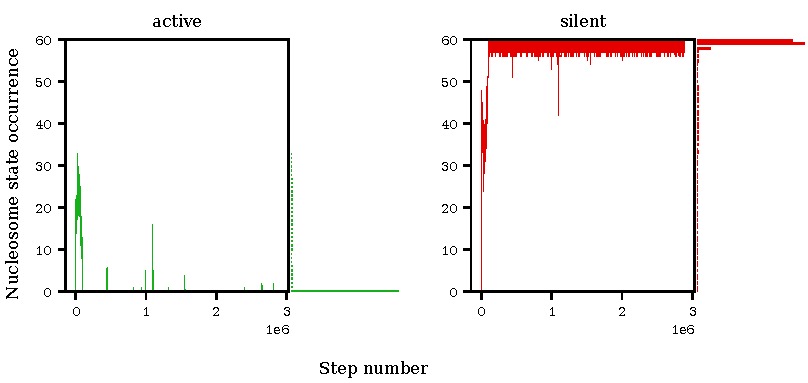
\includegraphics[width=\textwidth]{Results/4.1.1/peculiarCase4_0_runHistoryPlot_edited.pdf}
                        % \label{}
                    \end{minipage}
                \end{minipage}
                \begin{minipage}{\textwidth}
                    \begin{minipage}{0.1\textwidth}
                        \caption*{\small \textbf{(b)}}
                    \end{minipage}
                    \begin{minipage}{0.85\textwidth}
                        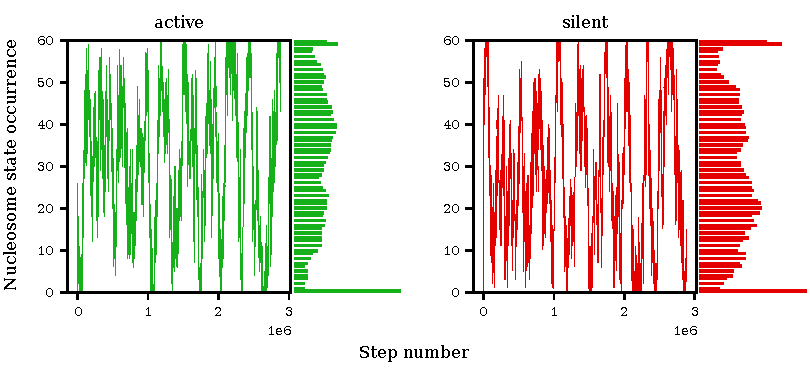
\includegraphics[width=\textwidth]{Results/4.1.1/peculiarCase2_edited.pdf}
                    \end{minipage}
                \end{minipage}
                \begin{minipage}{\textwidth}
                    \begin{minipage}{0.1\textwidth}
                        \caption*{\small \textbf{(c)}}
                        % \label{}
                    \end{minipage}
                    \begin{minipage}{0.85\textwidth}
                        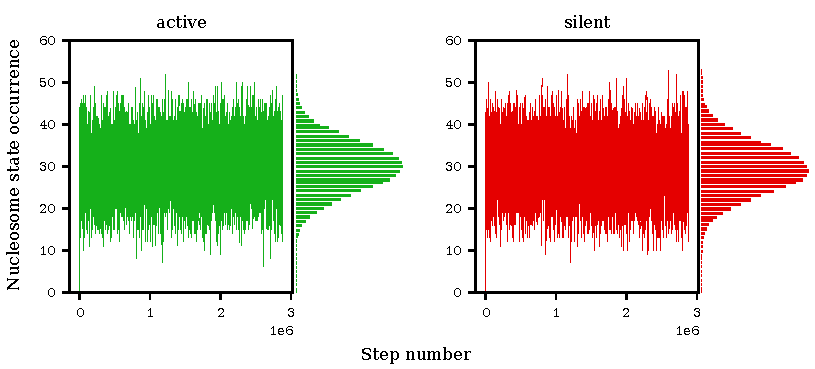
\includegraphics[width=\textwidth]{Results/4.1.1/peculiarCase3_1_runHistoryPlot_edited.pdf}
                        % \label{}
                    \end{minipage}
                \end{minipage}
                \caption{Absolute number of nucleosome states (active in green, silent in red) during the course of one long simulation (about 3 million reaction steps). Only every 1000th step is depicted. The enzyme rule set contains linear adders, random adders and random removers. The rule set does not contain cooperative enzymes. The enzymes' association rates are — linear adders: 40000 (20000 to each side), random removers: 2 and random adders: \textbf{(a)} 1, \textbf{(b)} 100, \textbf{(c)} 10000}
                \label{img:nonCoopSim}
            \end{figure}
            %

            %
            \begin{figure}[t!]
                \centering
                \includerunplot{Results/4.1.1/higherRandRemoverRates.pdf}
                \caption{Absolute number of nucleosome states (active in green, silent in red) during the course of one long simulation (about 4 million reaction steps). The enzyme rule set contains linear adders, linear removers, random adders and random removers. The rule set does not contain cooperative enzymes.}
                \label{img:nonCoopSim_bonus}
            \end{figure}
            %

            %
            In case \textbf{(a)} of fig. \ref{img:nonCoopSim}, at very low noise levels, one can easily see that the predominant state (here the silencing one) is stabilized. That said, no bistability is observed per se. However, it was found in additional simulation runs that the active state could just as easily turn out as the predominant state for the entire run. This fact seems rather logical as the starting state is a completely unmodified string and the used enzyme rule set is purely symmetrical, which means that it does not lean towards any of the two states concerning the association and dissociation rates.
            %

            %
            In case \textbf{(b)}, after increasing noise levels, the lack of resistance against noise gets clearer. As there are clearly two sharply defined most prevalent states with the chromatin string either fully acetylated or fully methylated, it might be tempting to call the system bistable. However, in sum, the states in between these extreme states are populated much more often, which makes the bistability in this system quite weak and not really applicable as something resembling a switch in a biological system.
            %

            %
            Finally, in case \textbf{(c)} with the random adders' association rate as close as $\nicefrac{1}{4}$ of the linear adders' and therefore considerably high noise levels, no bistability whatsoever can be observed any more. The histogram which counts the occurrence of active and silent nucleosomes respectively within the string shows a unimodal distribution throughout the simulation which is a “random walk”-like pattern on a fully modified string. The string is fully-modified because the dissociation rates are high compared to the association rates. The random modifications originate from overwhelming activity of the random enzymes. Accordingly, the nucleosome string states achieved during the simulation indeed disclose a monostable system.
            %

            %
            Increasing the random removers' rates results in more noise as well. This can be seen in fig. \ref{img:nonCoopSim_bonus} where the same enzyme rule set as in case \textbf{(b)} of fig. \ref{img:nonCoopSim} was used, except that the random removers' rates were raised from 2 to 100. In this case, the random walk area seems to have grown bigger and the string's full methylation or acetylation have both become extremely unstable.
            %
        %
        %
        \subsection{Bistability through indirect cooperativity}
            \label{subsec:indirectCoop}
            %

            %
            In a system of exclusively non-cooperative enzymes  with association rates indicated in table \ref{img:enzymeRatesPeculiarCase}, quite frequent bistability can indeed occur by adding linear removers to the rule set that was used in the example above.
            %

            %
            \begin{table}[htbp!]
                \caption{Enzyme types that are included in the rule set for the run illustrated in fig. \ref{img:outlook_nonCoop} with their respective association rates. All enzymes' dissociation rates are at an equal rate of 100,000. The enzyme rule set is symmetrical, which means that every enzyme type exists in favour of acetylation as well as methylation at equal rates respectively.}
                \begin{center}
                    \begin{tabular}{l r}
                        \hline
                        \textbf{enzyme type} & \textbf{association rate} \\
                        \hline
                        random adder & 100 \\
                        random remover & 2 \\
                        linear adder & 40,000 (20,000 to either direction)\\
                        linear remover & 40,000 (20,000 to either direction)\\
                        \hline
                    \end{tabular}
                \end{center}
                \label{img:enzymeRatesPeculiarCase}
            \end{table}
            %

            %
            \begin{figure}[htpb!]
                \centering
                \includerunplot{Results/4.1.2/StrongExtenders_cyclic_1_runHistoryPlot.pdf}
                \caption{Absolute number of nucleosome states (active in green, silent in red) during the course of one long simulation (about 1 million reaction steps). The enzyme rule set contains linear adders, linear removers, random adders and random removers. The rule set does not contain cooperative enzymes.}
                \label{img:outlook_nonCoop}
            \end{figure}
            %

            %
            The state adoption in this system resembles bistable behaviour as can be seen in fig. \ref{img:outlook_nonCoop}. One can clearly see that there are two very distinct peaks at complete activation and complete silencing of the nucleosome string.
            %

            %
            This bistability is most probably due to the fact that this system can now achieve indirect cooperativity. In a first step one, the linear remover reads two next-neighbour nucleosomes of opposite modification and, upon dissociation, leaves one of these unmodified. In step two, a linear adder modifies this nucleosome (through the usual read and write process) after reading a modified nucleosome next to it. This two-step process involves three nucleosomes in total which fulfills the condition for indirect cooperativity. It remains debatable if it is important, if the “read-only” nucleosomes are really different ones or if they may even be one and the same, resulting in the total involvement of merely two nucleosomes.\\
            %

            %
            Even though this system is bistable, however, it shows lack of variance around the peaks in the histogram.
            %

            %
            The histogram's peak variance can be understood as the area where the system has a more or less strong tendency to return to the peak's state.
            %

            %
            This behaviour is not observed in the indirectly cooperative case described in fig. \ref{img:outlook_nonCoop}. Thus, one single opposite modification added randomly to the string might entail the system's return to a random walk. As the term “stability” describes a state's resistance against small deviations and the addition of one single modification is nothing more than an atomic deviation for this system, one can say that this indirectly cooperative case does not qualify as a really robustly bistable system.
            %

            %
            Nonetheless, it is an interesting phenomenon overall, as it remains a theoretically useful switch-like concept that might find use in the biological context.
            %
            %
        %
        %
    %
    %
    \clearpage
    \section{Direct cooperativity and bistability on a non-cyclic string}
        \label{sec:ResNonCyc}
        %
        \subsection{Impact of cooperative enzymes}
            \label{subsec:impactOfCooperativeEnzymes}
            %
            Contrarily to section \ref{sec:ResNon-cooperative}, the simulations described in this section do contain cooperative adders and removers in the enzyme sets. In order to keep the rule sets as simple as possible, linear adders and removers are excluded from the enzyme set. Accordingly, other than cooperative enzymes, the rule set only contains random adders and removers.
            %

            %
            \begin{figure}[htpb!]
                \centering
                \includerunplot{Results/3.2_nonCyclString/shortRun_nonCyclic_highDiss_wCoopRem_4_runHistoryPlot.pdf}
                \caption{Absolute number of nucleosome states (active in green, silent in red) during the course of one simulation (about 56000 reaction steps). The enzyme rule set contains cooperative adders, cooperative removers, random adders and random removers. The amount of reaction steps is significantly lower than in fig. \ref{img:nonCoopSim} in order to be able to plot the heatmaps in figs. \ref{img:nonCyclBistability_bindingNumbers} and \ref{img:nonCyclBistability_bindingTimeDuration} with the data set from the same simulation.}
                \label{img:nonCyclBistability_runPlot}
            \end{figure}
            %

            %
            \begin{figure}[htpb!]
                \centering
                \includeheatmap{Results/3.2_nonCyclString/shortRun_nonCyclic_highDiss_wCoopRem_4_bindingNumbers}
                \caption{Heatmap depicting the absolute numbers of enzyme associations per enzyme and per nucleosome on the nucleosome string. The numbers originate from the same simulation plotted in fig. \ref{img:nonCyclBistability_runPlot}.}
                \label{img:nonCyclBistability_bindingNumbers}
            \end{figure}
            %

            %
            \begin{figure}[htpb!]
                \centering
                \includeheatmap{Results/3.2_nonCyclString/shortRun_nonCyclic_highDiss_wCoopRem_4_bindingTimeDuration}
                \caption{Heatmap depicting the average enzyme binding duration per enzyme and per nucleosome on the nucleosome string. The duration is defined as the number of time steps the enzyme has bound to one and the same nucleosome without dissociation event taking place in between divided by the total simulation time. The numbers originate from the same simulation plotted in fig. \ref{img:nonCyclBistability_runPlot}.}
                \label{img:nonCyclBistability_bindingTimeDuration}
            \end{figure}
            %

            %
            Figs. \ref{img:nonCyclBistability_runPlot}, \ref{img:nonCyclBistability_bindingNumbers} and \ref{img:nonCyclBistability_bindingTimeDuration} are derived from one same simulation with an enzyme rule set that contains the two cooperative enzyme types.
            %

            %
            One can easily see in fig. \ref{img:nonCyclBistability_runPlot} that with the newly added enzymes the predominant state (here the silencing one) is stabilized. It was found in additional simulation runs (see appendix \ref{app:additionalRuns}) that the active state might just as easily be the predominant state for the entire run, comparable to the indirect cooperativity case explained in \ref{subsec:indirectCoop}.
            %

            %
            It is important to note, that the histogram in fig. \ref{img:nonCyclBistability_runPlot} shows some variance around the peaks which is an important condition for robust stability in the mathematical sense, contrarily to the findings in \ref{subsec:indirectCoop}. In other words, the nucleosome string resists small perturbations and is able to return to a state that mostly contains one type of modifications, which will from now on be called a \textit{complete} state.
            %

            %
            These facts, the system either \textit{stably} finding itself in a completely active as well as a completely silent state, show that robust bistability has been achieved with this enzyme set.\\
            %

            %
            Figs. \ref{img:nonCyclBistability_bindingNumbers} and \ref{img:nonCyclBistability_bindingTimeDuration} provide more insights into the underlying mechanisms of the system. They originate from the same data as fig. \ref{img:nonCyclBistability_runPlot} does. As for the notion of 'space' indicated for each cooperative enzyme, please refer to section \ref{subsubsec:coopEnzymes}. A few seemingly surprising factors are to be addressed here.
            %

            %
            Every cooperative enzyme type shows a trapeze-like shape originating from a decreasing writeable area on the string with increasing pattern reach. This observation is tied to the inability of the enzymes to look beyond the string borders. As the pattern size increases, the cooperative enzyme is more and more unable to write onto a nucleosome  increasingly further away from the border. This is an unwanted effect, as it remains doubtful if this reflects any behaviour that would be seen as such in a natural biological setting.\\
            %

            %
            Fig. \ref{img:nonCyclBistability_bindingTimeDuration} reveals that there is a big discrepancy between the binding time of some enzymes compared to others. As the dissociation rates of the enzymes are very high and, importantly, precisely equal for every enzyme, completely dark spots must mean, that no enzyme has been active on that specific nucleosome at all throughout this simulation. For instance, the cooperative acetylation adders only seem to have been active on some nucleosomes close to both borders. The rest of the variance must originate from the stochastic nature of the simulation. Thus, this kind of plot is very useful for determining, if an enzyme type has been active at all on a specific nucleosome.\\
            %

            %
            Referring to fig. \ref{img:nonCyclBistability_bindingNumbers}, it is clear to see that the absolute number of associations of the random methylation remover is quite constant on most of the nucleosomes. As \ed/ was used as simulation tool, it is made sure that there are no associations without a following reaction and dissociation. Thus, as the random modification remover's context is one single modified nucleosome, the association number of the random removers can be taken as a locator of the modification (i.e. methylation or acetylation) they are removing with quite acceptable efficiency. In other words, fig. \ref{img:nonCyclBistability_bindingNumbers}, which shows the amount of enzyme associations per enzyme and per nucleosome, directly indicates, where a modification type was most prevalent on the string.
            %

            %
            The methylation mark was predominant throughout the entirety of the simulation. Given that the mentioned adders and removers are most active the more acetylation marks are already on the string, it does not seem surprising that the cooperative acetylation adders and the cooperative methylation removers show relatively low activity. The interesting activity pattern of those two enzyme types suggests that the acetylation subpopulations that can be seen in fig. \ref{img:nonCyclBistability_runPlot} must have been prevalent at the borders of the string almost exclusively. This is supported by the fact that the random methylation remover shows reduced activity at the borders.
            %

            %
            Thus can be concluded that it is very unlikely for any acetylation area to occur in the middle of the string while methylation is predominant, because empty spaces originating from random methylation removers are immediately filled up by cooperative methylation adders. The borders of the string, however, have a blocking effect on the cooperative methylation adders because with increasing space value, the nearest nucleosome that can be modified by them moves further and further away from the string border. The very first and very last nucleosomes are not modifiable at all by cooperative enzymes, hence the generation of acetylation subpopulations on the string borders.
            %
            %
        %
        %
        \subsection{Bistable switching on a non-cyclic string}
            %
            Considering the biological implications of the system, it would be much more useful if the system could effectively switch from one state to another within the course of one simulation, i.e. without changing the enzyme types involved or their rates and without resetting the nucleosome string to a completely unmodified string.
            %

            %
            This \textit{bistable switching} phenomenon, although rare, can be observed with the rule set described above (see fig. \ref{img:nonCyclBistability_runPlot2}). With the rule set containing random adders, removers and cooperative adders and removers, the system shows a bimodal distribution originating from one single simulation. Bistable switching can be observed about once every 10th simulation. Among hundreds of simulations, very few showed more than one bistable switching.
            %

            %
            As can be seen in fig. \ref{img:nonCyclBistability_runPlot2} between the times 0.2 and 0.4, the system undergoes bistable switching rather slowly. It is quite hard to determine any points of no return on the upper or lower border of this saddle point.
            %

            %
            \begin{figure}[htpb!]
                \centering
                \includerunplot{Results/3.2_nonCyclString/shortRun_nonCyclic_highDiss_wCoopRem_2_runHistoryPlot.pdf}
                \caption{Absolute number of nucleosome states (active in green, silent in red) during the course of one simulation (about 56000 reaction steps). Every reaction step is depicted in the plot. The x-axis shows the reaction time given by Gillespie's algorithm. The enzyme rule set contains cooperative adders, cooperative removers, random adders and random removers. Bistable switching, as seen in the plot, is only observed in about every 10th simulation of comparable reaction step size. The amount of reaction steps is significantly lower than in fig. \ref{img:nonCoopSim} in order to be able to plot the heatmaps in figs. \ref{img:coopAssocBindingDuration} and \ref{img:coopAssocBindingNumbers} with the data set from the same simulation.}
                \label{img:nonCyclBistability_runPlot2}
            \end{figure}
            %

             %
             \begin{figure}[htpb!]
                \centering
                \includeheatmap{Results/3.2_nonCyclString/shortRun_nonCyclic_highDiss_wCoopRem_2_bindingTimeDuration}
                \caption{Heatmap depicting the average enzyme binding duration per enzyme and per nucleosome on the nucleosome string. The duration is defined as the number of time steps the enzyme has bound to one and the same nucleosome without dissociation event taking place in between divided by the total simulation time. The numbers originate from the same simulation plotted in fig. \ref{img:nonCyclBistability_runPlot2}.}
                \label{img:coopAssocBindingDuration}
            \end{figure}
            %

            %
            \begin{figure}[htpb!]
                \centering
                \includeheatmap{Results/3.2_nonCyclString/shortRun_nonCyclic_highDiss_wCoopRem_2_bindingNumbers}
                \caption{Heatmap depicting the absolute numbers of enzyme associations per enzyme and per nucleosome on the nucleosome string. The numbers originate from the same simulation plotted in fig. \ref{img:nonCyclBistability_runPlot2}.}
                \label{img:coopAssocBindingNumbers} 
            \end{figure}
            %

            %
            In fig. \ref{img:coopAssocBindingDuration}, the main difference from fig. \ref{img:nonCyclBistability_bindingTimeDuration} in the previous subsection is that both cooperative adders have been active across the entirety of the string in the present simulation, which makes sense because both modifications were predominant at one point in time.
            %

            %
            As can be seen in fig. \ref{img:coopAssocBindingNumbers}, the random remover enzymes are by far the most active enzymes from the set in this simulation, followed by the random adder enzymes which mainly show activity at the string borders. Apart from the random enzymes, the cooperative acetylation adders were active across the whole string while the other cooperative enzymes only were most active at the borders. Another interesting detail is that the cooperative methylation adders' activity looks a little stronger from nucleosome 30 onward to 60 than on the other half of the string. This behaviour could be recreated several times in other simulations where bistable switching occurred.
            %

            %
            As already pointed out in \ref{subsec:impactOfCooperativeEnzymes}, the acetylation mark must have taken over starting from the string borders, hence the intense enzymatic activity at these areas. The asymmetrical activity level of the cooperative methylation adders is particularly indicative of how and from where exactly the acetylation mark must have taken over. As the system reaches the saddle point, the acetylation area must probably have progressed all the way to the centre of the string from the left (i.e. nucleosome 1) rendering the cooperative methylation adder particularly inactive in this area for \nicefrac{1}{5} of the simulation time. It is likely that the opposite effect was not seen on the cooperative acetylation adders' activity pattern because the acetylation modification is prevalent for a longer time span (about \nicefrac{3}{5}), whereas the predominance period of the methylation modification is about as long as the system's prevalence periods in  proximity to the saddle point (about \nicefrac{1}{5}). These fraction indications are consistent even when looking at the absolute reaction step numbers. They are not distorted by the event-based time incrementation of Gillespie's algorithm.
            %
        %
        %
        \subsection{Bivalent switching on a non-cyclic string}
            %

            %
            In other simulations with the same settings as above (i.e. same enzyme rule set, starting state and simulation parameters), both modification levels meet close to the saddle point around 30 nucleosomes for quite a while before one modification turns out to be the predominant state again.
            %

            %
            \begin{figure}[htpb!]
                \centering
                \includerunplot{Results/3.2_nonCyclString/321_longRun_nonCyclic_highDiss_wCoopRem_01_runHistoryPlot.pdf}
                \caption{Absolute number of nucleosome states (active in green, silent in red) during the course of one simulation (about 175000 reaction steps). Every reaction step is depicted in the plot. The x-axis reaction step number. The enzyme rule set contains cooperative adders, cooperative removers, random adders and random removers.}
                \label{img:nonCyclBistability_runPlot3}
            \end{figure}
            %

            %
            The macrostate switching phenomenon shown in fig. \ref{img:nonCyclBistability_runPlot3} cannot be described as a "direct transition", which disqualifies it from being bistable switching (as it was defined in \ref{sec:TheoBistableSwitching}). Much rather, this phenomenon could be described as \textit{bivalent switching}, where the area around the saddle point is the pseudostable “STANDBY” state from which the system can evolve in either a completely active or silent macrostate. Clearly, the idea of \textit{irreversibility} (originating from the observation of bivalency in the context of generally unidirectional cell differentiation) is not reflected in this system.
            %

            %
            \begin{figure}[htpb!]
                \centering
                \includeheatmap{Results/3.2_nonCyclString/321_longRun_nonCyclic_highDiss_wCoopRem_01_bindingNumbers}
                \caption{Heatmap depicting the absolute numbers of enzyme associations per enzyme and per nucleosome on the nucleosome string. The numbers originate from the same simulation plotted in fig. \ref{img:nonCyclBistability_runPlot3}.}
                \label{img:coopAssocBindingNumbers_runPot3}
            \end{figure}
            %

            %
            In fig. \ref{img:coopAssocBindingNumbers_runPot3}, an asymmetrical activity pattern can be seen for the cooperative \ac/ adders as well as the random \ac/ removers. Both were quite a bit more active from nucleosome position 1 to 30 than on the other half of the chromatin string, while the random \me/ remover shows the exact opposite pattern. Again, given that the SSA does not allow dissociation without preoccuring reaction, it is certain to say that the left (1 - 30) half of the chromatin string contained \ac/ modifications more often throughout the simulation, while the right (31 - 60) half contained \me/ modifications more often.
            %

            %
            Like before, it is convenient to conclude that as soon as the saddle point was reached, there were two quite clearly separated areas present on the string: the \ac/ modification on one side and the \me/ modification on the other leaving both modifications at about equal possibility of taking over to be the predominant macrostate.
            %

            %
            Many of the phenomena discussed in this section originated from the linearity of the nucleosome string. As such, it presents two borders which, as was pointed out, have massive impacts on the enzymes' activity and also bistability. As these borders hardly seem justifiable from a biological point of view, it would be interesting and much more relevant biologically to achieve bistable switching on a nucleosome string without borders. This will be examined in the next section.
            %

            %
        %
        %
    %
    %
    \clearpage
    \section{Bistable switching on a cyclic string}
        \label{sec:ResBistableSwitching}
        %

        %
        \subsection{Achieving bistable switching}
            %
            %
            As was pointed out before, a linear nucleosome string with a finite number of nucleosomes that is reduced of length because of computational feasibility might not be best when aiming at designing a most general model that shows bistable switching. The drawbacks due to border effects of such a non-cyclic chain are evident as of the previous sections.
            %

            %
            \begin{figure}[htpb!]
                \centering
                \includerunplot{Results/3.3_bistableSwitching/longRun_cyclic_highDiss_wCoopRem_1_runHistoryPlot.pdf}
                \caption{Absolute number of nucleosome states (active in green, silent in red) during the course of one long simulation (about 678 million reaction steps). Only every 1000th step is depicted. The enzyme rule set contains random adders, random removers, cooperative adders and cooperative removers.}
                \label{img:cyclWCoopRem_runPlot1}
            \end{figure}
            %

            %
            \ed/ provides a means to work with circular nucleosome chains by establishing a direct next-neighbour relationship between the very first and very last nucleosome in the string. This method was used from this point on in the rest of the work. As border effects could now be effectively excluded, the nucleosome string length was reduced from 60 to 40 in order to lower computation expenses. It was made sure that the enzymes' maximum reach in the system was always low enough in order for the reduced string length not to trigger interlacing effects.
            %

            %
            With the borders eliminated, no bistable switching could be observed any more (see fig. \ref{img:cyclWCoopRem_runPlot1}). After one of the 2 modification types turns out predominant, it stays like this throughout the simulation with very little variance. This was to be expected, as the string borders helped the non-predominant modification to stay on the string end in the first place before growing its area across up to the other end of the string. As was pointed out in the previous section, the cooperative removers are much too strong for a non-prevalent modification to survive long enough without the protecting borders.\\
            %

            %
            The logical next step was to remove the cooperative removers from the rule set altogether. As can be seen in figs. \ref{img:cyclBistability_runPlot1} and \ref{img:cyclBistability_runPlot2}, this step was decisive for obtaining bistable switching on a cyclic string.
            %

            %
            \begin{figure}[htpb!]
                \centering
                \includerunplot{Results/3.3_bistableSwitching/longRun_cyclic_highDiss_noCoopRem_1_runHistoryPlot.pdf}
                \caption{Absolute number of nucleosome states (active in green, silent in red) during the course of one long simulation (about 634 million reaction steps). Only every 1000th step is depicted. The enzyme rule set contains random adders, random removers and cooperative adders (no cooperative removers).}
                \label{img:cyclBistability_runPlot1}
            \end{figure}
            %

            %
            \begin{figure}[htpb!]
                \centering
                \includerunplot{Results/3.3_bistableSwitching/longRun_cyclic_highDiss_noCoopRem_2_runHistoryPlot.pdf}
                \caption{Absolute number of nucleosome states (active in green, silent in red) during the course of one long simulation (about 634 million reaction steps). Only every 1000th step is depicted. The enzyme rule set contains random adders, random removers and cooperative adders (no cooperative removers).}
                \label{img:cyclBistability_runPlot2}
            \end{figure}
            %

            %
            As can be seen in these two figs., the removal of the cooperative removers not only entails the reappearance of bistable switching. Moreover, bistable switching is much more frequent in the simulations so much so that even multiple switchings in one simulation are not rare events any more. One can also see that the histogram peaks moved a bit closer towards the axis centre of 20 which means that the most stable states are not complete states any more. Instead, there is always a considerable subpopulation of about 10\% of the opposite modification present, showing high variance.
            %

            %
            Although the system passes the saddle point around 20 nucleosomes quite often, it seems that this state is never populated for a very long time, as is shown by figs. \ref{img:cyclBistability_runPlot1} and \ref{img:cyclBistability_runPlot2}. Accordingly, the point of no return seems much more narrow than in the linear case with cooperative removers present in the rule set.\\
            %
            %
        %
        %

        \subsection{Length of macrostates}
            \label{subsec:macrostateLength}
            %
            %
            As bistable switching has become a quite common phenomenon in this setting, it seems tempting to calculate the average \textit{macrostate length}, with the macrostate defined as the current predominant modification state. In order to do so, for each simulation out of 150 with total step numbers of about 650,000 respectively, every macrostate length was counted. The macrostate started when at least 75\% of the nucleosomes on the string presented one same modification, and it ended when the opposite modification was present on 75\% of the nucleosomes. This implies that the “transition” states around the saddle point are included in the macrostate lengths. However, this was considered to be acceptable given that the transitions in this system are quite negligeable concerning their relative duration and the resulting inclusion of transition states is equally distributed for \me/ as well as \ac/ macrostates.
            %

            %
            Also, all macrostates that lasted up until the end of the simulation were not counted because the duration of said macrostates could not be accurately determined as their end was not yet reached at the end point of the simulation. Accordingly, macrostates from simulations which did not show any bistable switching were discarded.
            %

            %
            \begin{figure}[htpb!]
                \begin{minipage}{.69\textwidth}
                    \centering
                    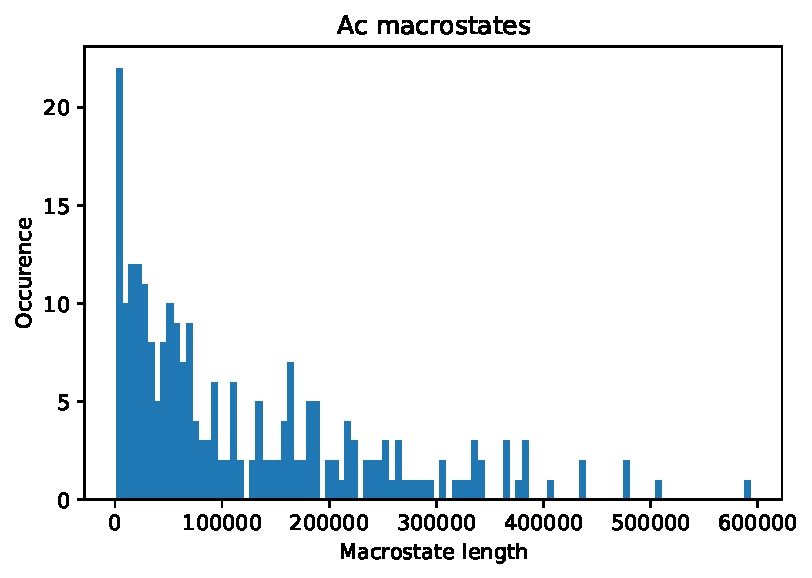
\includegraphics[width=\textwidth]{Results/3.3_bistableSwitching/macrostate_length_hist.pdf}
                    \caption*{\textbf{(a)}}
                \end{minipage}
                \begin{minipage}{.29\textwidth}
                    \centering
                    \begin{tabular}{rr}
                        count	& 243.000 \\
                        mean	& 119779.021 \\
                        % std	    & 118142.252 \\
                        min	    & 1180.000 \\
                        25\%	& 26212.500 \\
                        50\%	& 71719.000 \\
                        75\%	& 182782.000 \\
                        max	    & 593180.000 \\
                    \end{tabular}
                    \caption*{\textbf{(b)}}
                \end{minipage}
                \caption{\textbf{(a)} Histogram counting the acetylation macrostates' lengths of a system with identical settings as the one described at the beginning of this section. \textbf{(b)} Statistical data of the acetylated macrostates}
                \label{img:cyclBistability_hist}
            \end{figure}
            %

            %
            \noindent
            A data summary of the findings can be seen in fig. \ref{img:cyclBistability_hist}.
            %

            %
            With a total count of 243 bistable switchings throughout the 150 simulations, the data abundance is quite scarce on the considerable value range of about 1000 up to almost 600,000. Additionally, the mean value of about 119,779 seems quite far away from the most frequent value range, which makes an underlying Poisson distribution unlikely. Besides this, because of the high complexity of the collected data, it does not seem trivial to determine if the macrostate length is a Poisson process at all.
            %

            %
            Regardless, more data would be needed in order to be able to perform solid statistical analyses. However, achieving the needed amount of data seems unfeasible with the present computational and timely resources of the author.
            %
        %
        %
        \subsection{Enzyme contributions per macrostate}
            %
            %
            In order to get more insights into the macrostates' influence on the enzymes, the macrostate dependent activity of the random and cooperative adders was analysed by differentiating between three nucleosome string state categories: the \ac/ macrostate (>75\% of nucleosomes on the string are acetylated), the \me/ macrostate (>75\% of nucleosomes on the string are methylated) and the grey area closer around the saddle point which holds all other states. For convenience reasons, these three categories will be referred to as macrostates of the system which includes the grey area in this context.
            %

            %
            String states which show more than 25\% of unmodified nucleosomes were not taken into account. However, such cases were only discovered at the beginning of the simulation.
            %

            %
            For the macrostates separately, the adder enzyme counts were summarized over the same 150 simulations of around 600,000 simulation steps as above. The enzyme association rates are 140,000 for the cooperative adders (20,000 for every differently spaced rule), 10,000 for the random adders and 2 for the random removers. The percentage of enzymatic adder activity is summarized in tab. \ref{tab:cyclBistability_enzymes}.
            %

            %
            \begin{table}[htpb!]
                \centering
                \caption{Macrostate dependent adder enzyme binding event counts in percent. \textit{Me} refers to the \me/ macrostate, \textit{Ac} to the \ac/ macrostate and Grey refers to the state in-between the two macrostates, where both modifications are prevalent on less than 75\% of the nucleosomes.}
                \begin{tabular}{lrrrrr}
                                &   CoopM	    &   CoopA       &   RandM       &   RandA   &   $\Sigma$  \\\hline
                    Me	        &   21.00\%	    &   0.21\%	    &   1.86\%	    &   1.85\%   &   24.91\%    \\
                    Grey        &   10.44\%	    &   10.49\%	    &   3.17\%	    &   3.18\%   &   27.28\%    \\
                    Ac	        &   0.21\%	    &   21.00\%	    &   1.85\%	    &   1.86\%   &   24.92\%    \\
                \end{tabular}
                \label{tab:cyclBistability_enzymes}
            \end{table}
            %

            % % equal amount of significant numbers
            % \begin{table}[htpb!]
            %     \centering
            %     \caption{Macrostate dependent adder enzyme binding event counts in percent. \textit{Me} refers to the \me/ macrostate, \textit{Ac} to the \ac/ macrostate and Grey refers to the state in-between the two macrostates, where both modifications are prevalent on less than 75\% of the nucleosomes.}
            %     \begin{tabular}{lrrrrr}
            %         Macrostate  &   CoopM	    &   CoopA       &   RandM       &   RandA   &   $\Sigma$  \\\hline
            %         Me	        &   21.00	    &   0.2053	    &   1.856	    &   1.854   &   24.91    \\
            %         Grey        &   10.44	    &   10.49	    &   3.166	    &   3.184   &   27.28    \\
            %         Ac	        &   0.2066	    &   21.00	    &   1.853	    &   1.857   &   24.92    \\
            %     \end{tabular}
            %     \label{tab:cyclBistability_enzymes}
            % \end{table}
            %

            %
            It might seem surprising at first that for every state category (Me, Grey, Ac), the overall adder binding event percentage is only around 25\%. However, this makes perfect sense because every enzyme binding event is followed by a reaction/dissociation step which will make up for about another 25\% of the overall event count. The remaining 50\% are probably due to random remover binding and removing activity.
            %

            %
            Other than that, the enzymes show expected symmetrical activity levels: the random enzymes are equally active in the \me/ macrostate as in the \ac/ macrostate and the cooperative \me/ adder is equally active in the \me/ macrostate as the cooperative \ac/ adder is in the \ac/ macrostate and vice versa.
            %

            %
            \begin{table}[htpb!]
                \centering
                \caption{Macrostate dependent modification events in percent. \textit{Me} refers to the \me/ macrostate, \textit{Ac} to the \ac/ macrostate and Grey refers to the state in-between the two macrostates, where both modifications are prevalent on less than 75\% of the nucleosomes.}
                \begin{tabular}{lrr}
                                &   Methylation	    &   Acetylation \\\hline%\hline
                    Me	        &   91.36\%	        &   8.26\% \\%\hline
                    Grey        &   49.86\%	        &   50.14\% \\%\hline
                    Ac	        &   8.27\%	        &   91.73\% \\
                \end{tabular}
                \label{tab:cyclBistabilities_modificationProb}
            \end{table}
            %

            %
            Tab. \ref{tab:cyclBistabilities_modificationProb} summarizes the respective \ac/ and \me/ modification rates for each macrostate based on the data from tab. \ref{tab:cyclBistability_enzymes}. Understandably, methylation and acetylation events happen at equal rates in the grey area, as the system can establish either \me/ or \ac/ macrostates from the saddle point. The rate of about 8\% of acetylation events in the \me/ macrostate (and vice versa) are consistent with the previous graphical estimation, that the respective subpopulations are to find on about 10\% of nucleosomes.
            %

            %
            \begin{table}[htpb!]
                \centering
                \caption{Macrostate dependent contributions of cooperative and random adders respectively in percent. \textit{Me} refers to the \me/ macrostate, \textit{Ac} to the \ac/ macrostate and Grey refers to the state in-between the two macrostates, where both modifications are prevalent on less than 75\% of the nucleosomes.}
                \begin{tabular}{l|rr|rr}
                                &   \multicolumn{2}{|c|}{Methylation}    & \multicolumn{2}{c}{Acetylation} \\
                                &   random	    &   cooperative     &   random      &   cooperative     \\\hline%\hline
                    Me	        &   8.12\%	    &   91.88\%         &   90.00\%     &   9.96\%  \\%\hline
                    Grey        &   23.28\%	    &   76.72\%         &   23.28\%     &   76.72\% \\%\hline
                    Ac	        &   89.95\%	    &   10.05\%         &   8.12\%      &   91.88\% \\
                \end{tabular}
                \label{tab:cyclBistabilities_enzymeProb}
            \end{table}
            %

            %
            Tab. \ref{tab:cyclBistabilities_enzymeProb} further breaks down the numbers in order to show the contributions of the different enzyme types, random and cooperative, for the respective macrostate. It is easier to see here that the numbers for methylation are equal to the inverted acetylation numbers.
            %

            %
            It was to expect that in all the macrostates, the effective association ratio between the cooperative adder and the random adder activity is different from the set one, because the cooperative enzymes' pattern includes more restrictions. Theoretically, given that the cooperative adders have a set association rate of 140,000 and the random adders' association rate is set at 10,000, one could expect that the random enzymes bind at least $\nicefrac{1}{14}$ as often as the cooperative adders. This is indeed observed for all three macrostates.
            %

            %
            Interestingly, the cooperative enzymes are about three times as active as the random adders in the grey area and still show an activity of $\nicefrac{1}{10}$ in the respective non-favoured macrostate. One would expect that, in an \ac/ dominated macrostate for instance, a cooperative \me/ adder might be able to read its pattern far less often given that the \me/ modification is only present in a relatively small subpopulation. A possible explanation is that the modifications are scattered very randomly along the chromatin string, in contrast to the non-cyclic case.
            %
            %
        %
        %
    %
    %
    \newpage
    \section{The boundaries of bistability}
        \label{sec:ResBoundariesBistability}
        %

        %
        \subsection{Influence of the dissociation rate}
            \label{subsec:ResInfluenceDissociationRate}
            %

            %
            In the previous sections, the system's parameter that was most focussed on were the enzyme types in the rule set. The dissociation rate, however, was kept at a very high rate. This section serves the purpose of examining, what happens if the dissociation events enter in concurrence with the associations throughout the simulation.
            %

            %
            \begin{figure}[htpb!]
                \centering
                \includerunplot{Results/3.4_dissocRate/longRun_cyclic_lowDiss_noCoopRem_3_runHistoryPlot_wSum.pdf}
                \caption{Absolute number of nucleosome states (active in green, silent in red, sum of active and silent in blue) during the course of one long simulation (about 126 million reaction steps). Only every 1000th step is depicted. The enzyme rule set contains random adders, random removers and cooperative adders (no cooperative removers).}
                \label{img:dissoc_runPlot1}
            \end{figure}
            %

            %
            \begin{figure}[htpb!]
                \centering
                \includerunplot{Results/3.4_dissocRate/longRun_cyclic_highDiss_noCoopRem_3_runHistoryPlot_wSum.pdf}
                \caption{Absolute number of nucleosome states (active in green, silent in red, sum of active and silent in blue) during the course of one long simulation (about 639 million reaction steps). Only every 1000th step is depicted. The enzyme rule set contains random adders, random removers and cooperative adders (no cooperative removers).}
                \label{img:dissoc_runPlot2}
            \end{figure}
            %

            %
            In the previous simulations, enzymes were bound for an average of two or three events before writing and dissociating from the bound nucleosome. Decreasing the dissociation rate inherently means a longer binding time on the nucleosome. Fig. \ref{img:dissoc_runPlot1} shows that this longer binding time entailed by a lower dissociation rate (100) has severe effects on the whole simulation outcome compared to a simulation with exactly the same parameters except for a 1000 times higher dissociation rate (100,000) for every enzyme (see fig. \ref{img:dissoc_runPlot2}).
            %

            %
            Fig. \ref{img:dissoc_runPlot1} discloses a much lower number of total reaction events during the simulation from fig. \ref{img:dissoc_runPlot1} compared to fig. \ref{img:dissoc_runPlot2}. Additionally, the most striking difference is that the adopted states histogram shows a monomodal distribution even though it is easy to see from fig. \ref{img:dissoc_runPlot2} that a bimodal distribution and, thus, bistability can be achieved with this enzyme set.
            %

            %
            It is evident that bistability, although possible from a rule set point of view, can be eliminated by a low dissociation rate. This is probably because during binding time, the enzymes are blocking the ability for other enzymes to bind to the same nucleosome and, in a way, act as protective groups. As a result, the number of possible events for each respective time step is massively reduced. This is also shown by the reduced overall event number in fig. \ref{img:dissoc_runPlot1}, as the SSA increases the time elapsed between events the lower the number of possible events is (see \ref{subsec:Gillespie}).
            %

            %
            An additional striking detail from fig. \ref{img:dissoc_runPlot1} is that the total number of modified nucleosomes is generally quite low compared to fig. \ref{img:dissoc_runPlot2}. It averages around 25 out of 40 nucleosomes which means that at any time during the simulation, around 15 nucleosomes on the string are unmodified. This probably happens because many association events are followed by reaction and dissociation rather lately.
            %

            %
            The protective behaviour of enzymes with low dissociation rate and the high number of unmodified nucleosomes are likely to be the main reasons for bistability not occuring in simulations with enzymes that have low dissociation rates. Cooperative adders are meant to take the dominating modification into account to act as the main drivers for bistability. With low dissociation rates, the presence of quite many unmodified nucleosomes as well as a slowed down modification velocity because of protective enzymes inhibit the cooperative adders and, thus, prevent bistability.
            %

            %
            Thus, it seems that the dissociation rate is an important influential factor that has to be taken into account or “eliminated” by raising its value high enough when trying to achieve bistability.
            %
        %
        %
        \subsection{Cooperative enzyme reach}
            \label{subsec:cooperativeEnzymeReach}
            %
            Another interesting property is the cooperative enzymes' reach , i.e. the space between the reading areas and the writing position.
            %

            %
            \begin{figure}[htpb!]
                \centering
                \begin{minipage}{0.77\textwidth}
                    \begin{minipage}{0.1\textwidth}
                        \caption*{\small \textbf{(a)}}
                        % \label{}
                    \end{minipage}
                    \begin{minipage}{0.65\textwidth}
                        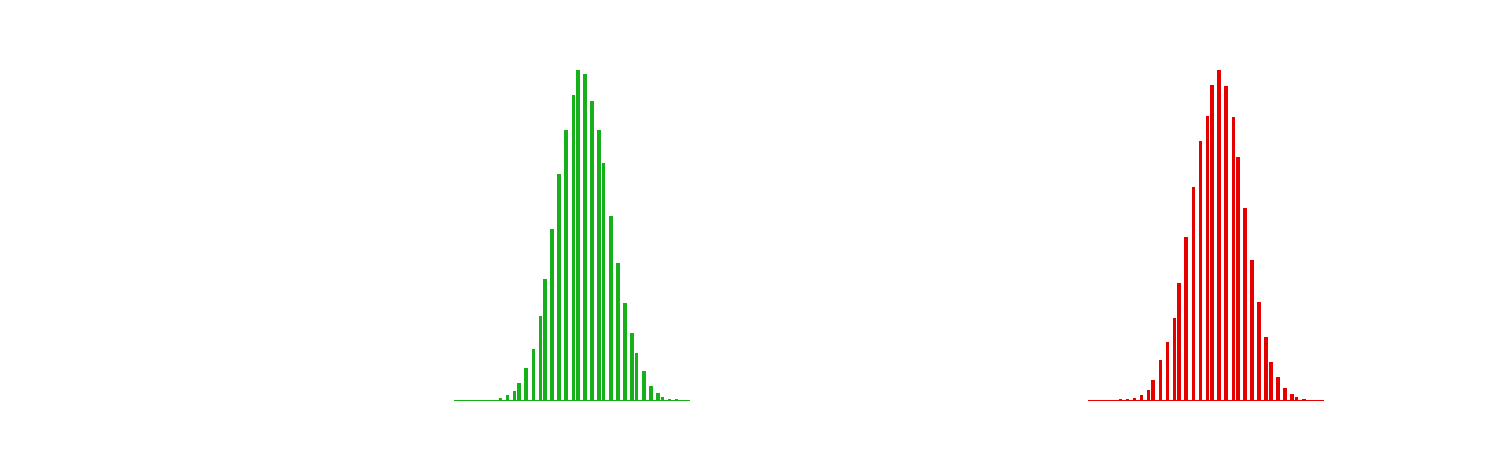
\includegraphics[width=\textwidth]{Results/3.5_boundariesBistability/maxReach0_0_HistogramPlot.pdf}
                        % \label{}
                    \end{minipage}
                \end{minipage}
                \begin{minipage}{0.77\textwidth}
                    \begin{minipage}{0.1\textwidth}
                        \caption*{\small \textbf{(b)}}
                    \end{minipage}
                    \begin{minipage}{0.65\textwidth}
                        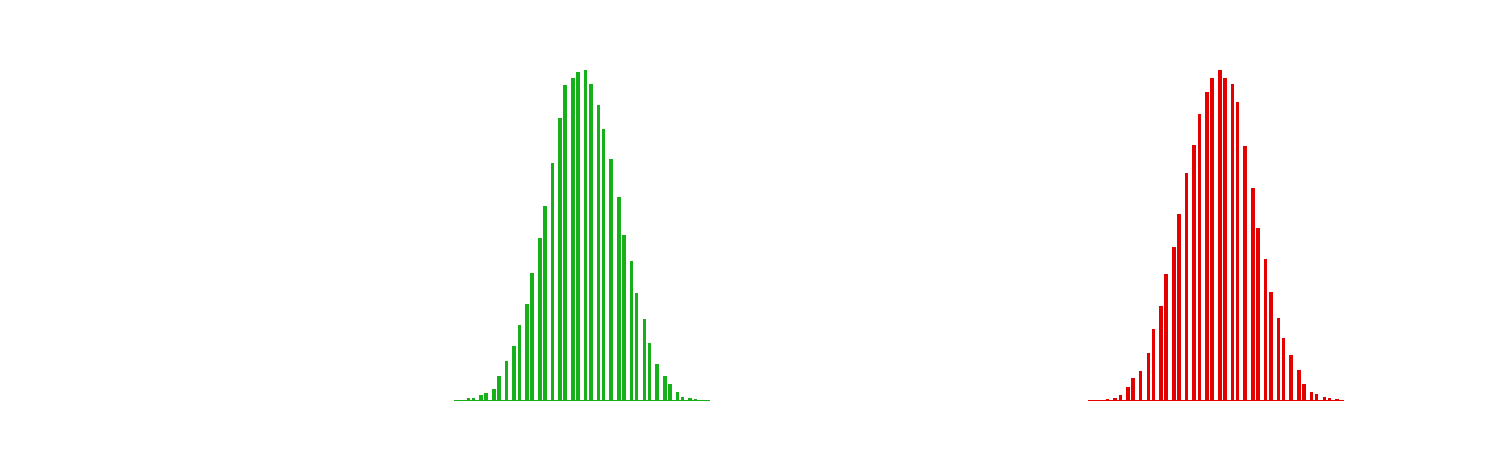
\includegraphics[width=\textwidth]{Results/3.5_boundariesBistability/maxReach1_4_HistogramPlot.pdf}
                    \end{minipage}
                \end{minipage}
                \begin{minipage}{0.77\textwidth}
                    \begin{minipage}{0.1\textwidth}
                        \caption*{\small \textbf{(c)}}
                        % \label{}
                    \end{minipage}
                    \begin{minipage}{0.65\textwidth}
                        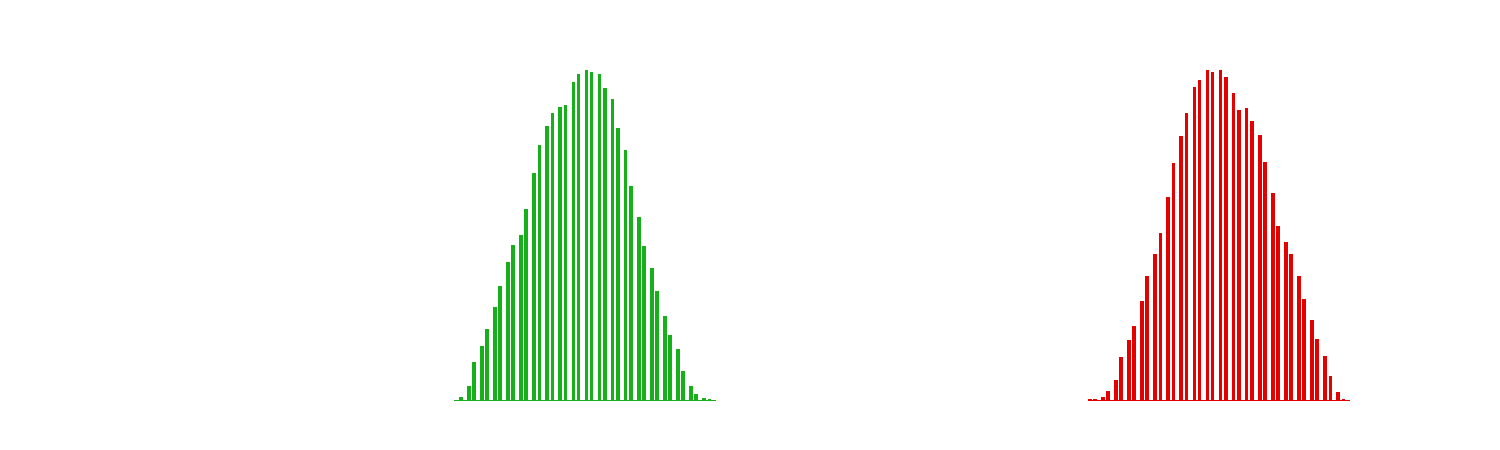
\includegraphics[width=\textwidth]{Results/3.5_boundariesBistability/maxReach2_2_HistogramPlot.pdf}
                        % \label{}
                    \end{minipage}
                \end{minipage}
                \begin{minipage}{0.77\textwidth}
                    \begin{minipage}{0.1\textwidth}
                        \caption*{\small \textbf{(d)}}
                    \end{minipage}
                    \begin{minipage}{0.65\textwidth}
                        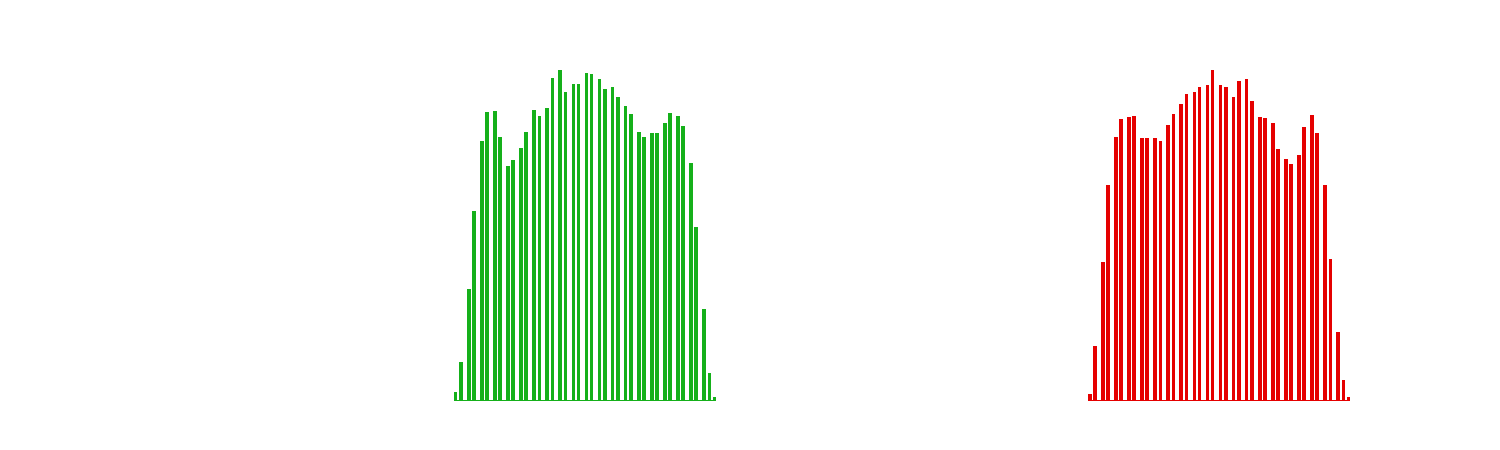
\includegraphics[width=\textwidth]{Results/3.5_boundariesBistability/maxReach3_3_HistogramPlot.pdf}
                    \end{minipage}
                \end{minipage}
                \begin{minipage}{0.77\textwidth}
                    \begin{minipage}{0.1\textwidth}
                        \caption*{\small \textbf{(e)}}
                        % \label{}
                    \end{minipage}
                    \begin{minipage}{0.65\textwidth}
                        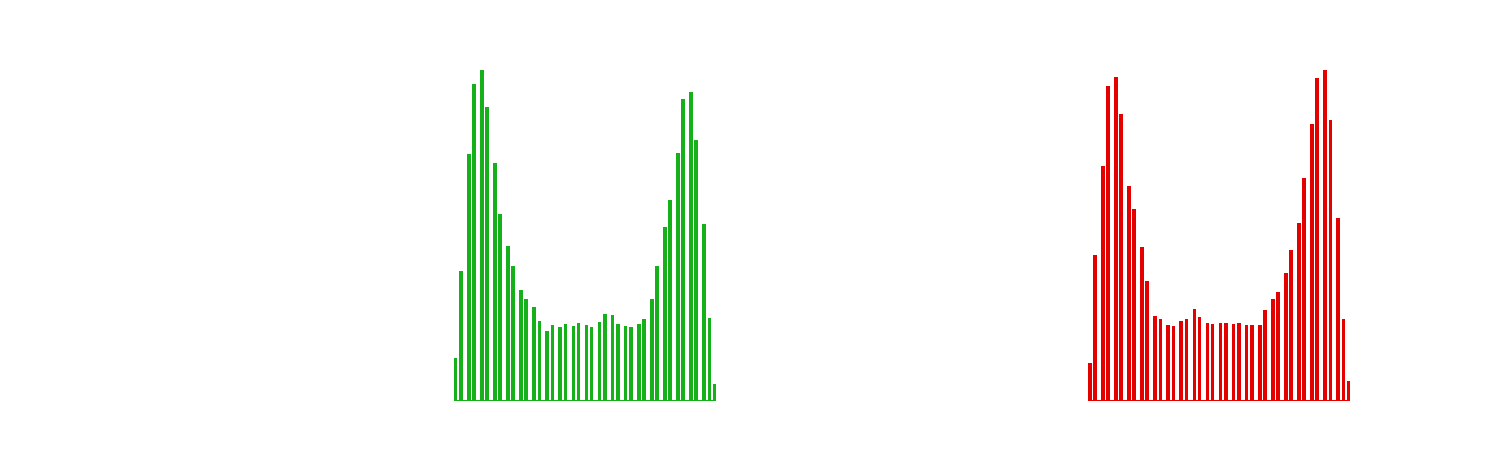
\includegraphics[width=\textwidth]{Results/3.5_boundariesBistability/maxReach4_3_HistogramPlot.pdf}
                        % \label{}
                    \end{minipage}
                \end{minipage}
                \begin{minipage}{0.77\textwidth}
                    \begin{minipage}{0.1\textwidth}
                        \caption*{\small \textbf{(f)}}
                    \end{minipage}
                    \begin{minipage}{0.65\textwidth}
                        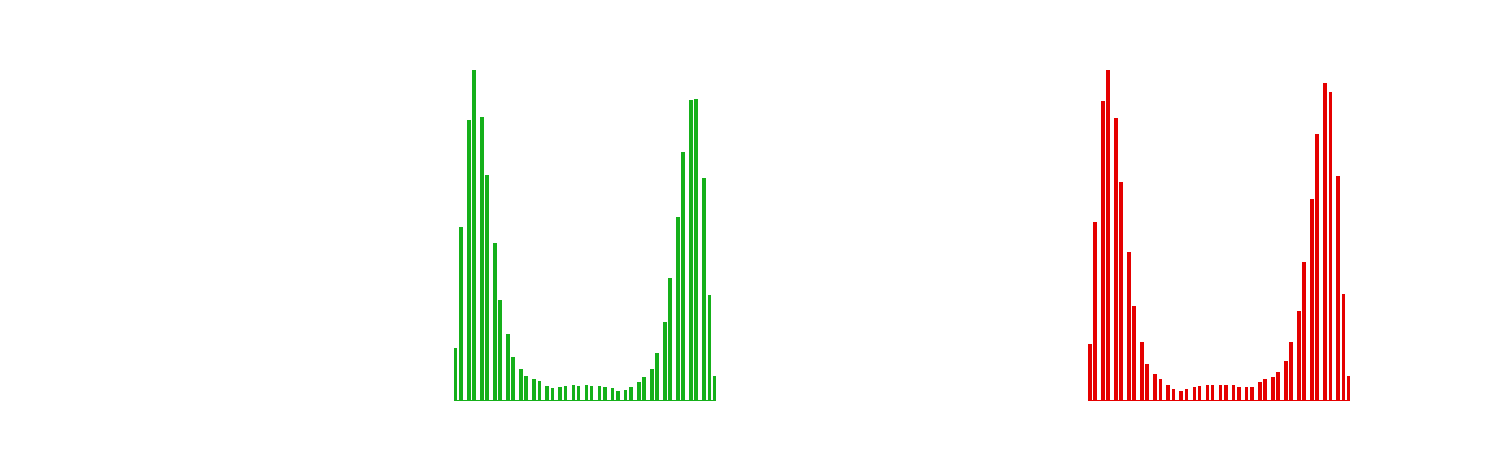
\includegraphics[width=\textwidth]{Results/3.5_boundariesBistability/maxReach5_4_HistogramPlot.pdf}
                    \end{minipage}
                \end{minipage}
                \begin{minipage}{0.77\textwidth}
                    \begin{minipage}{0.1\textwidth}
                        \caption*{\small \textbf{(g)}}
                    \end{minipage}
                    \begin{minipage}{0.65\textwidth}
                        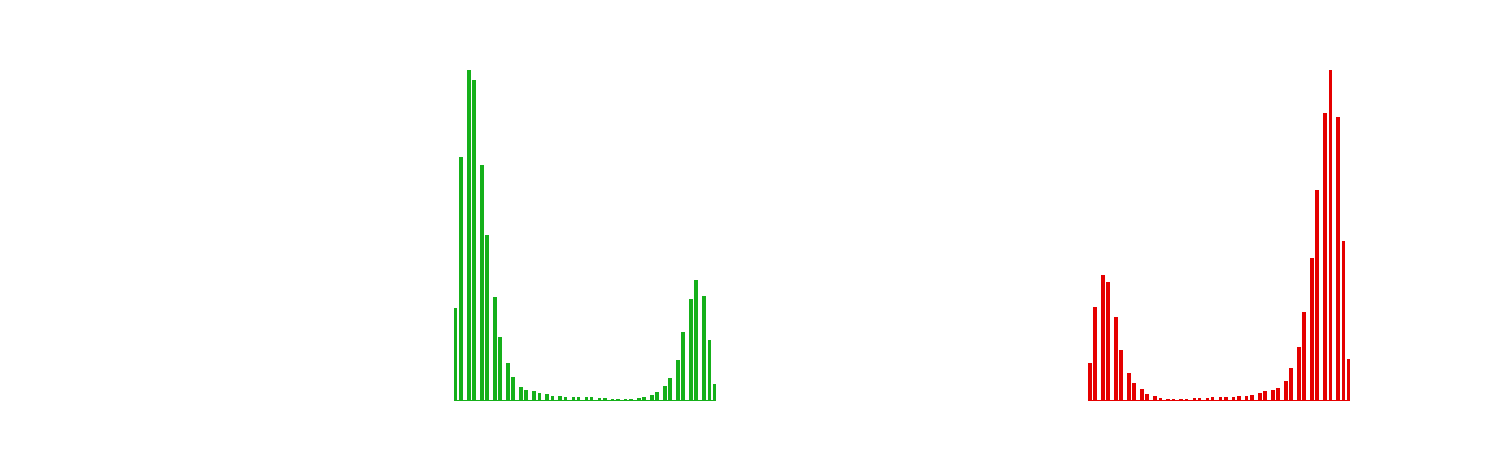
\includegraphics[width=\textwidth]{Results/3.5_boundariesBistability/maxReach6_4_HistogramPlot.pdf}
                    \end{minipage}
                \end{minipage}
                \caption{Histograms representing the absolute number of nucleosome states from 40 (left) to 0 (right) (active in green, silent in red, sum of active) during the course of one long simulation (about 638 million reaction steps). The enzyme rule set contains random adders, random removers and cooperative adders (no cooperative removers). The cooperative adders' maximum space is varied to be \textbf{(a)} 0, \textbf{(b)} 1, \textbf{(c)} 2, \textbf{(d)} 3, \textbf{(e)} 4, \textbf{(f)} 5 and \textbf{(g)} 6. Space is defined as the number of nucleosomes between the nucleosome which is read on either side and the unmodified nucleosome that is to be modified. The space to the left and right is always equal for every respective cooperative adder rule.}
                \label{img:enzymeReach}
            \end{figure}
            %

            %
            In all previous sections, cooperative adders constantly included rules with spaces of zero up to six. Space is defined as the number of nucleosomes between a “read-only” nucleosome and the nucleosome to be modified. The space is equal left and right of the nucleosome to be modified.
            %

            %
            Fig. \ref{img:enzymeReach} shows that the histograms of the absolute nucleosome state numbers change dramatically when varying the cooperative adders' space variable. Case \textbf{(a)} shows a monomodal distribution, which is to be expected because the cooperative adders in this system do not have a pattern that exceeds next-neighbour relations. As explained in \ref{subsec:multistable}, this fact makes bistability very hard up to impossible to achieve at considerable noise levels. It seems that for the present set of parameters, including the chromatin length of 40 nucleosomes, the present association rates of 140,000 (20,000 for each space rule) for cooperative adders, 10,000 for random adders and 2 for random removers and a universal dissociation rate of 100,000, a bimodal distribution is consistently achieved starting at a space of 4, as can be seen in case \textbf{(e)} of fig. \ref{img:enzymeReach}. In this case, the cooperative adders' biggest pattern contains 11 nucleosomes, including the nucleosome to be modified, having an overview across $\nicefrac{1}{4}$ of the entire nucleosome string.
            %

            %
            Naturally, no general statement can be given based on these findings as to how far cooperative adders with fixed “arm” lengths have to be able to “detect” modifications. However, it has become clear that fixed neighbour relations are not an unbreachable barrier when trying to achieve robust bistability or even bistable switching, provided the reach is far enough.
            %

            %
            Another interesting effect can be seen in cases \textbf{(e)}, \textbf{(f)} and \textbf{(g)}. For one, the saddle point seems less and less populated with increasing enzyme reach. Secondly, case \textbf{(g)} shows an asymmetrical distribution which might not be expected at first. Summarizing those two observations, it seems that the macrostates turn out to gain stability the higher the cooperative enzymes' reach is. As a result, one macrostate lasts longer than the other one in a simulation which results in an asymmetrical bimodal distribution. For example, in case \textbf{(g)} from fig. \ref{img:enzymeReach}, the active macrostate prevailed longer than the silent macrostate. Overall, the system is still symmetrical, as there are also simulations based on identical parameters which show the opposite picture with the silent macrostate being the longer lasting one.
            %

            %
            When choosing an even larger space value for the cooperative adders, the macrostates become more and more stable up to a point where bistable switching can only rarely be observed any more. As some simulations still show an acetylation macrostate whereas others show a methylation macrostate, the system is still bistable, regardless of the space value, provided the latter is above the value of four.
            %
            %
        %
        %
    %
    %
    % \newpage
    % \section{Bivalency}
    %     \label{sec:ResBivalency}
    %     %
    %     \begin{figure}[htpb!]
    %         \centering
    %         \includerunplot{Results/3.6_Bivalency/TotalComplete_example.png} % change this
    %         \caption{}
    %         % \label{img:dissoc_runPlot2}
    %     \end{figure}
    %     %
    %     \begin{figure}[htpb!]
    %         \centering
    %         \includerunplot{Results/3.6_Bivalency/BivalentComplete_example.png} % change this
    %         \caption{}
    %         % \label{img:dissoc_runPlot2}
    %     \end{figure}
    %     %
    %     \begin{figure}[htpb!]
    %         \centering
    %         \includerunplot{Results/3.6_Bivalency/BivalentBistability_example.png} % change this
    %         \caption{}
    %         % \label{img:dissoc_runPlot2}
    %     \end{figure}
    %     %
    %     \begin{itemize}
    %         {
    %             \color{red} %
    %             \item Here, we are at Kx+Ky
    %             \item Two systems that either favour bivalency or total active/silent states as an introduction to bivalency
    %             \item Frequent switching and bivalency
    %         }
    %     \end{itemize}
        %
    %
    %
%
%